\documentclass[tikz,border=6pt]{standalone}
\usepackage[T1]{fontenc}
\usepackage[utf8]{inputenc}
\usepackage{pgfplots}
\usepgfplotslibrary{groupplots}
\usetikzlibrary{calc}
\pgfplotsset{compat=1.18}
\begin{document}
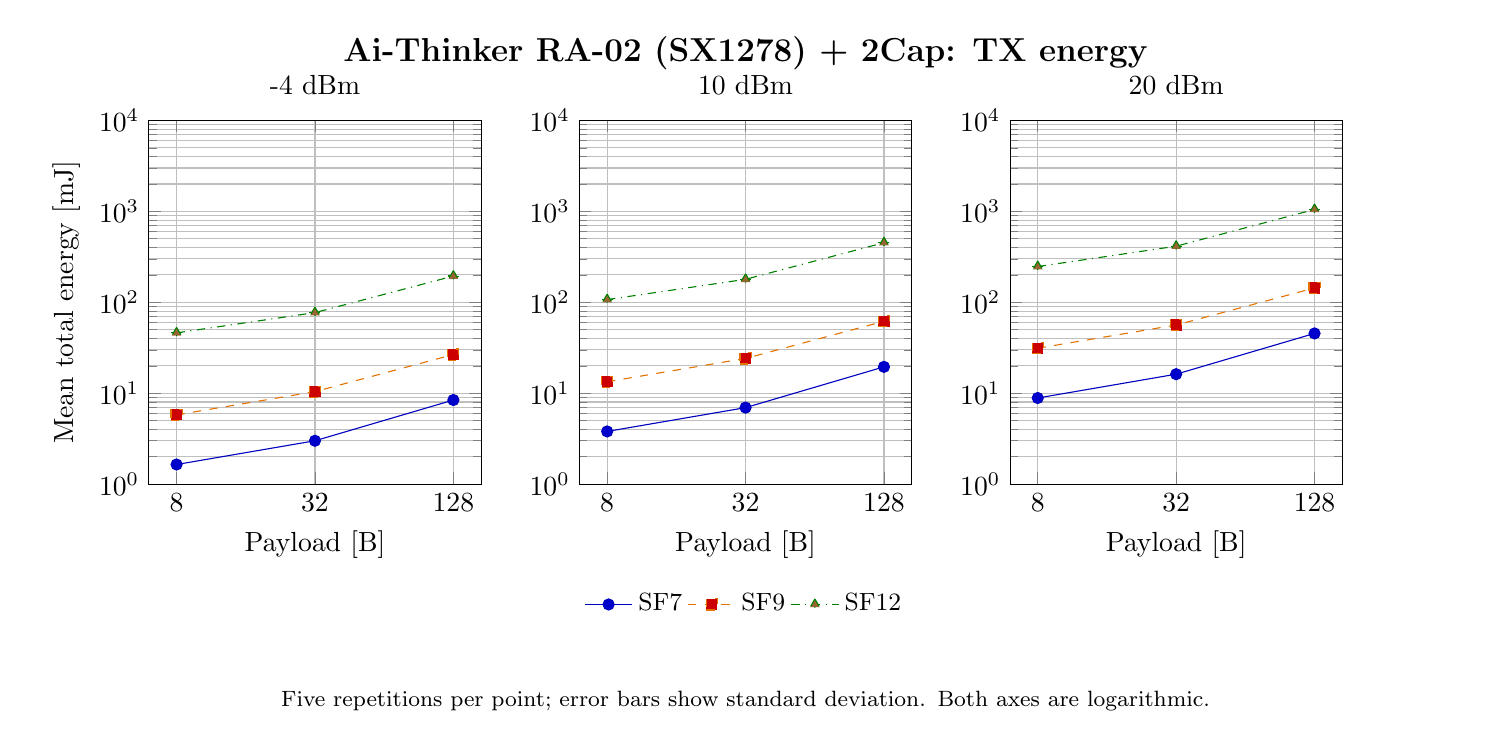
\begin{tikzpicture}
\begin{groupplot}[/pgf/number format/use comma, group style={group size=3 by 1, horizontal sep=1.25cm},
  width=5.8cm,height=6.2cm,xmode=log,log basis x=2,ymode=log,log basis y=10,ymin=1,ymax=10000,
  xtick={8,32,128},xticklabels={8,32,128},grid=both,xlabel={Payload [B]},
  legend style={draw=none,fill=none,font=\small,at={(0.5,-0.27)},anchor=north,legend columns=-1}]
% TX energy
\nextgroupplot[title={-4 dBm},ylabel={Mean total energy [mJ]}]
\addplot+[blue!75!black,solid,mark=*,error bars/.cd,y dir=both,y explicit] coordinates {(8,1.64124127) +- (0,0.00279445544) (32,2.99454351) +- (0,0.00456197605) (128,8.40574446) +- (0,0.0133984902)};
\addplot+[orange!90!black,dashed,mark=square*,error bars/.cd,y dir=both,y explicit] coordinates {(8,5.76814821) +- (0,0.0103813723) (32,10.3956949) +- (0,0.0268351229) (128,26.586662) +- (0,0.0457173948)};
\addplot+[green!50!black,dashdotted,mark=triangle*,error bars/.cd,y dir=both,y explicit] coordinates {(8,46.0463088) +- (0,0.0277843353) (32,76.9274057) +- (0,0.0579390494) (128,194.079731) +- (0,0.260467975)};
\nextgroupplot[title={10 dBm}]
\addplot+[blue!75!black,solid,mark=*,error bars/.cd,y dir=both,y explicit] coordinates {(8,3.79317841) +- (0,0.00641491013) (32,6.93181506) +- (0,0.00551039923) (128,19.469495) +- (0,0.0190310601)};
\addlegendentry{SF7}
\addplot+[orange!90!black,dashed,mark=square*,error bars/.cd,y dir=both,y explicit] coordinates {(8,13.3546108) +- (0,0.0141624329) (32,24.1038629) +- (0,0.0189798926) (128,61.687432) +- (0,0.0380029082)};
\addlegendentry{SF9}
\addplot+[green!50!black,dashdotted,mark=triangle*,error bars/.cd,y dir=both,y explicit] coordinates {(8,106.916323) +- (0,0.0389838349) (32,178.755622) +- (0,0.0677947748) (128,451.58515) +- (0,0.278989889)};
\addlegendentry{SF12}
\nextgroupplot[title={20 dBm}]
\addplot+[blue!75!black,solid,mark=*,error bars/.cd,y dir=both,y explicit] coordinates {(8,8.84459217) +- (0,0.0628122301) (32,16.1710185) +- (0,0.0760864794) (128,45.4043796) +- (0,0.234788619)};
\addplot+[orange!90!black,dashed,mark=square*,error bars/.cd,y dir=both,y explicit] coordinates {(8,31.2249375) +- (0,0.171757926) (32,56.2012148) +- (0,0.361300725) (128,143.588993) +- (0,0.663372236)};
\addplot+[green!50!black,dashdotted,mark=triangle*,error bars/.cd,y dir=both,y explicit] coordinates {(8,246.9808) +- (0,0.355324712) (32,413.462779) +- (0,1.3359441) (128,1048.34669) +- (0,1.85065565)};
\end{groupplot}
\node[font=\bfseries\large] at ($(group c2r1.north)+(0,0.85cm)$) {Ai-Thinker RA-02 (SX1278) + 2Cap: TX energy};
\node[font=\footnotesize,align=center,text width=18cm] at ($(group c2r1.south)+(0,-2.75cm)$) {Five repetitions per point; error bars show standard deviation. Both axes are logarithmic.};
\end{tikzpicture}
\end{document}
